\clearpage
\section{Multimodal Machine Learning}

The aim of this thesis is to detect road defects using multimodal machine learning. As described earlier in section \ref{section:multimodal-ml}, multimodal means that there are multiple data sources. In this case, it deals with visual- and accelerometer data. There are three points in the pipeline where the modalities can be fused: early- middle- or late fusion \cite{Baltrusaitis2017}. However, a model can also be trained on the respective modality, i.e. training a classifier solely on visual data. This makes sense as it can act as a baseline to multimodal learner. Therefore this thesis researches three tracks:
\begin{enumerate}
\item Visual only: based on the visual data an object detector is trained to classify road anomalies.
\item Accelerometer only: based on the vibrations a model is trained to classify road anomalies.
\item Fusion: based on both modalities a model is trained. All three strategies of fusion are evaluated.
\end{enumerate}


\begin{figure}[ht]
\begin{center}
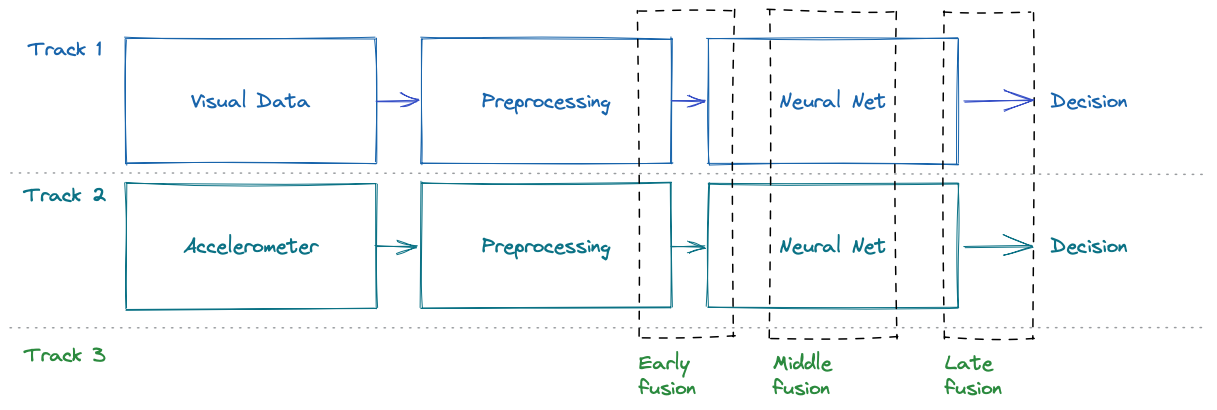
\includegraphics[width=0.95\textwidth,keepaspectratio]{images/5_multimodal_fusion/fusion-strategies.png}
\captionsetup{width=.95\textwidth}
\caption{Different tracks of detecting road surface defects. The moment of different fusion strategies are highlighted.}
\label{fig:fusion-strategies}
\end{center}
\end{figure}


\subsection{General Experiment Setup}
Experiments in subsequent sections are all ran on the same machine. This machine has the following specifications: Intel Core i7-7700K CPU, NVIDIA GeForce GTX 1080 GPU and 32 GiB RAM. The machine runs on Debian 11 as operating system. Experiments are tracked with an open-source tool called Weights and Biases (wandb) \cite{wandb}.

TODO: frame experiments as Action Design Research cycles


\subsection{Capture Time Synchronization}
\label{sec:capture-time-synchronization}


\subsection{Distance Estimation}
\label{sec:object-distance}


\subsection{Moment Filtering}


\subsection{Manhole Detection}
Trained three models, at 100 epochs
\begin{itemize}
\item $YOLO_v5s$ at 1280 with batch 8
\item $YOLO_v5m$ at 1280 with batch 4
\item $YOLO_v5m$ at 640 with batch 16
\end{itemize}

The models with higher resolution (1280) perform relatively equal but much better than with the lower input size. Therefore we continue training only on larger inputs. 

As the 1280 models are performing pretty similar, it makes sense to continue working with the s version. This YOLO model is smaller (less weights), but trains much quicker (86 min vs 226). 

\subsection{Track 1: Detecting Road Anomalies with Visual Data}

The first track is to train a model solely using visual data for detecting road anomalies. Road anomalies are basically objects in an image, thus framing the learning task as object detection: classifying and locating objects in an image. As we know from literature survey (refer back to \ref{sec:object-detection}), YOLOv5 \cite{Jocher2021} is regarded as the current state of the art model. The authors provide various kind of model configurations pre-trained on the COCO dataset. In this track, YOLO is used to detect manholes from the recorded video data.


\subsubsection{Evaluation Metrics}


An object detector returns for an image all the detected objects in the image. For each of the objects, the model returns the detected class, the confidence and the bounding box - that is where the object is located in the image. In order to determine if the model correctly classified a detected object, Intersection over Union (IoU) is used. It measures the overlap between the detected bounding box, and the ground truth (i.e. labelled) bounding box. IoU is calculated by the ratio of the area of intersection between the bounding boxes, over the total area of the bounding boxes, see also figure \ref{fig:iou}. When the IoU is above some threshold, the object is positively classified as that respective class.



\begin{figure}[ht]
\begin{center}
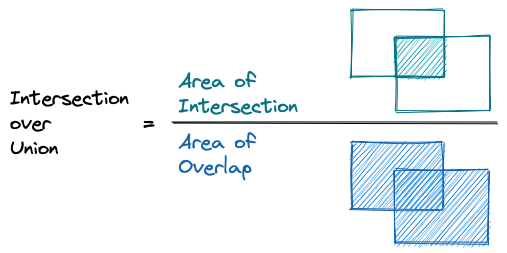
\includegraphics[height=4cm]{images/5_multimodal_fusion/IoU.png}
\end{center}
\captionsetup{width=0.95\textwidth}
\caption{Visualization describing the calculation of the Intersection over Union (IoU).}
\label{fig:iou}
\end{figure}



Object detectors are conventionally evaluated with mean Average Precision (mAP) \cite{Padilla2021}. In order to calculate it, the precision and recall of the model is evaluated for all object classes. Precision is calculated as the ratio of true positives over all predicted positives, $\text{Precision} = TP / (TP + FP)$, describing the correctness of classifications. Recall is calculated as the ratio of true positives over all actual positives, $\text{Recall} = TP / (TP + FN)$, describing the sensitivity of the model. Based on the configured threshold there is trade-off between precision and recall of a classifier. This can be visualized in a graph known as precision recall curve, see also figure \ref{fig:precision-recall-curve}. Average Precision (AP) is calculated as the area below the precision recall curve. Mean Average Precision (mAP) is basically the mean for all object classes of the AP.



\begin{figure}[ht]
\begin{center}
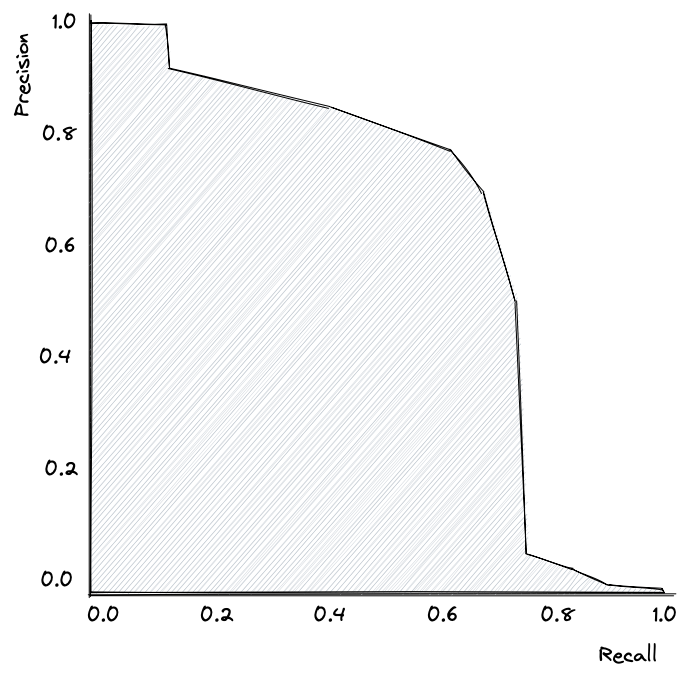
\includegraphics[height=4cm]{images/5_multimodal_fusion/precision-recall.png}
\end{center}
\captionsetup{width=0.95\textwidth}
\caption{Visualization describing the calculation of the Intersection over Union (IoU).}
\label{fig:precision-recall-curve}
\end{figure}


\subsubsection{Labelling}

As described earlier in section \ref{sec:visual-data}, the collected video data is extracted into frames. The video data is recorded at 30 frames per second. 

For this experiment data is manually labelled with a open-source tool called CVAT \cite{cvat}. 



In short, it compares the ground-truth bounding box to the detected box and returns a metric describing the precision. Where higher scores means a better detection. mAP is calculated 





\subsection{ADR Cycle 1: Detecting Roadside Location Markers}

With object detection the evaluation metrics measure how close the detected bounding boxes are to the ground-truth (labelled) bounding boxes. This measurement is done independently for each object class, by assessing the amount of overlap. Models are assessed on the following metrics: precision, recall and mAP \cite{Padilla2021}.

Precision is ability to identify only relevant objects, the percentage of correct predictions. Recall is ability to find all relevant cases, the percentage of correct predictions among all given ground truths. In practice, we want a good object detector that find all ground truth objects (high recall), while only identifying relevant objects (high precision). Average Precision (MP) is metric based on the area below Precision x Recall curve. AP is obtained for each individual class, to yield a single metric, mean average precision (mAP) can be calculated by averaging the AP over all classes \cite{Padilla2021}.

TODO: describe mAP calculation

The first experiment is to detect roadside location markers, also known as \textit{hectometerpaal} or \textit{mile marker}. These are  small signs that are along the road to indicate the current position. See also figure \ref{fig:road-indicator} for an example of Dutch road location marker. The task is to detect the location and orientation of road indicators from the gathered data. With this output we can determine if the road location marker is in good condition, e.g. it is not skewed backwards but clearly visible.

\begin{figure}[ht]
\begin{center}
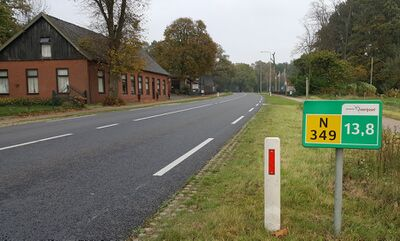
\includegraphics[height=4cm,keepaspectratio]{images/5_multimodal_fusion/example_hectometer.jpeg}
\end{center}
\caption{Example of roadside location marker (\textit{hectometerpaal}).}
\end{figure}


The reasons for this experiment are two-fold. First, the automation of detecting road sign damages. For road maintainers this is an easy optimization in their efficiency and thereby saves the road maintainers money. Second, although this is a relatively simple experiment, it enables the author to learn more about the practicalities of using YOLO, such as transfer learning, experiment tracking and resource utilization.


\subsubsection{Setup}
Classifying and locating objects is known as object detection. The output is the bounding box and class of the detected objects in an image. See also \ref{object-detection} for more information. Current state-of-the-art model for object detection is YOLOv5. This experiment uses YOLOv5 as model with pre-trained weights. The model is transfer learned to detect road side location markers. 

At this time there were 536 annotated frames with visible roadside location markers. The data comes from three different trips, filmed with the same camera. The frames are split into a training, validation and test split. With respective proportions of 70\% / 21\% / 9\%. 


\subsubsection{Results}
The following configurations are tested:


\begin{table}[h]
\begin{tabular}{lllllll}
Name                        & Model       & Image Size & Batch Size & Precision & Recall & mAP  \\
last\_95\_img-640\_batch-42 & UCS-InfoLab & 640        & 4          & 0.74      & 0.55   & 0.62 \\
yolo5m\_batch-640\_batch-4  & YOLOv5m     & 640        & 4          & 0.87      & 0.93   & 0.93 \\
yolo5s\_batch-640\_batch-32 & YOLOv5s     & 640        & 32         & 0.59      & 0.61   & 0.56 \\
yolo5s\_batch-640\_batch-16 & YOLOv5s     & 640        & 16         & 0.68      & 0.71   & 0.74 \\
yolo5s\_batch-640\_batch-8  & YOLOv5s     & 640        & 8          & 0.80      & 0.78   & 0.86 \\
yolo5s\_batch-1280\_batch-8 & YOLOv5s     & 1280       & 8           & \textbf{0.91} & \textbf{0.94} & \textbf{0.95}
\end{tabular}
\end{table}


\begin{figure}[h]
\begin{center}
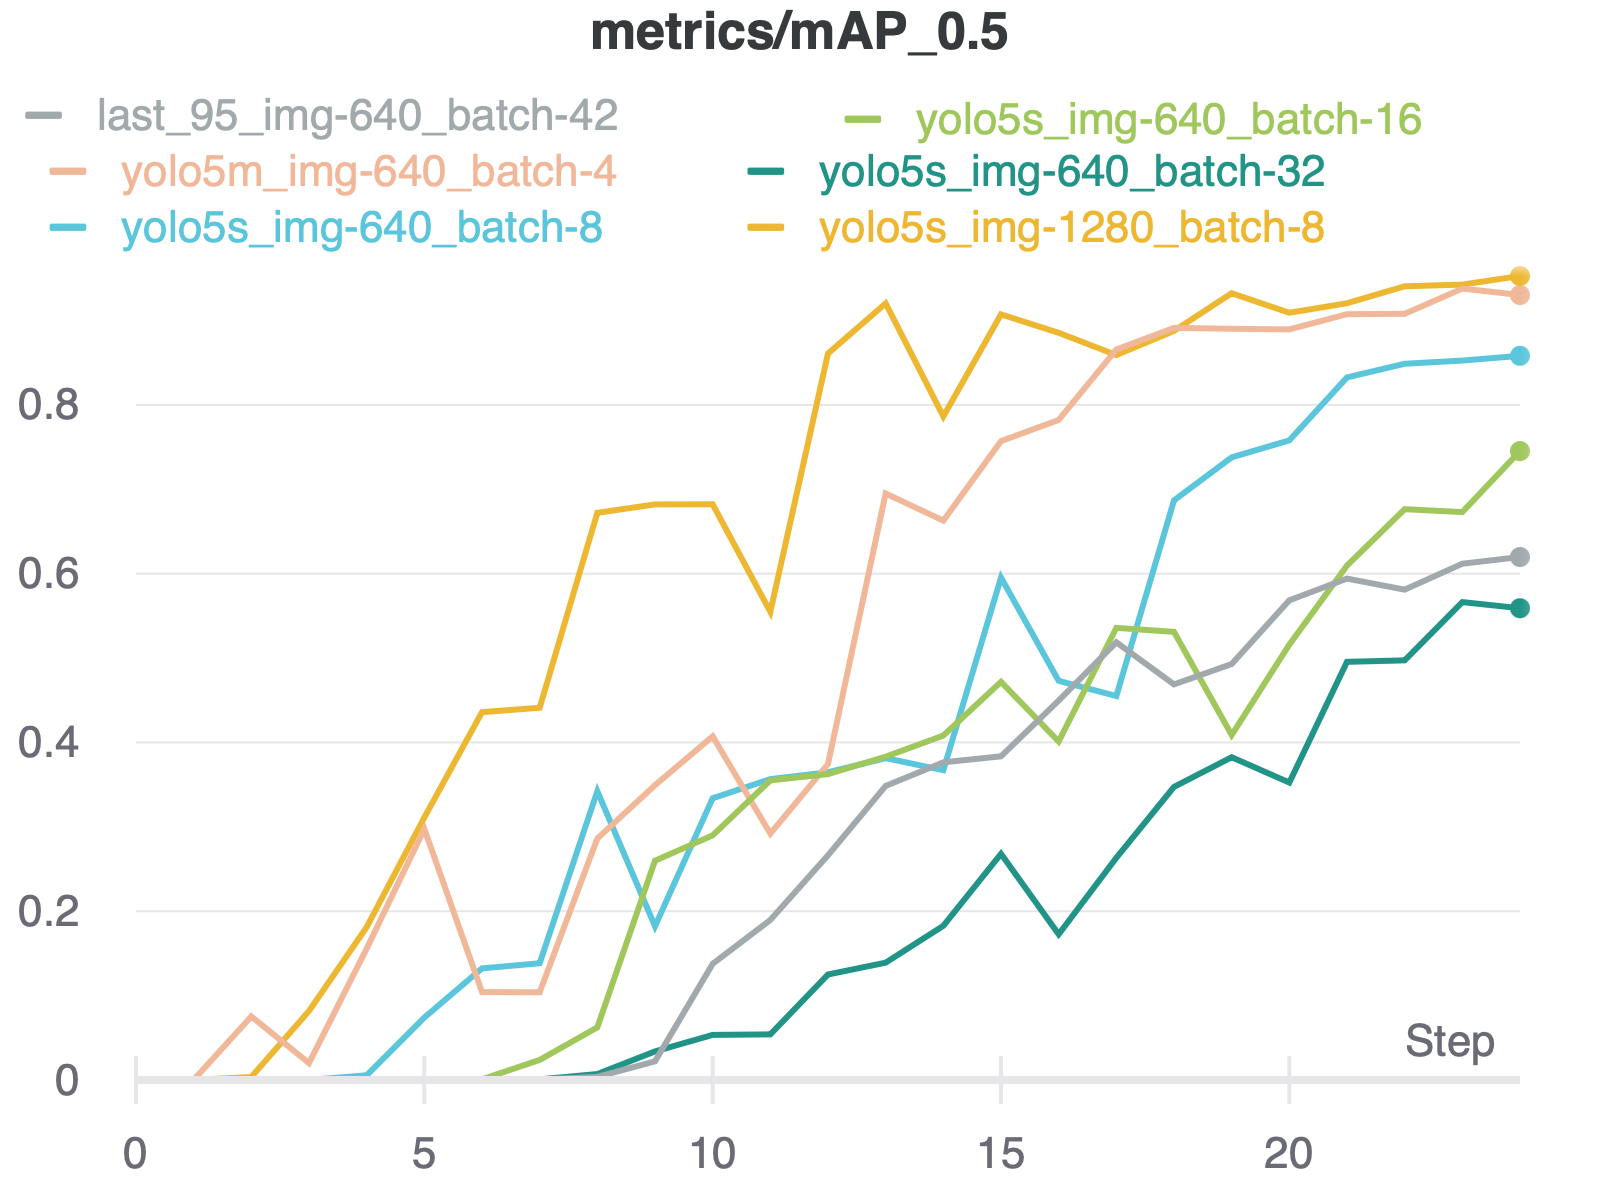
\includegraphics[height=4cm,keepaspectratio]{images/5_multimodal_fusion/exp-1_mAP.png}
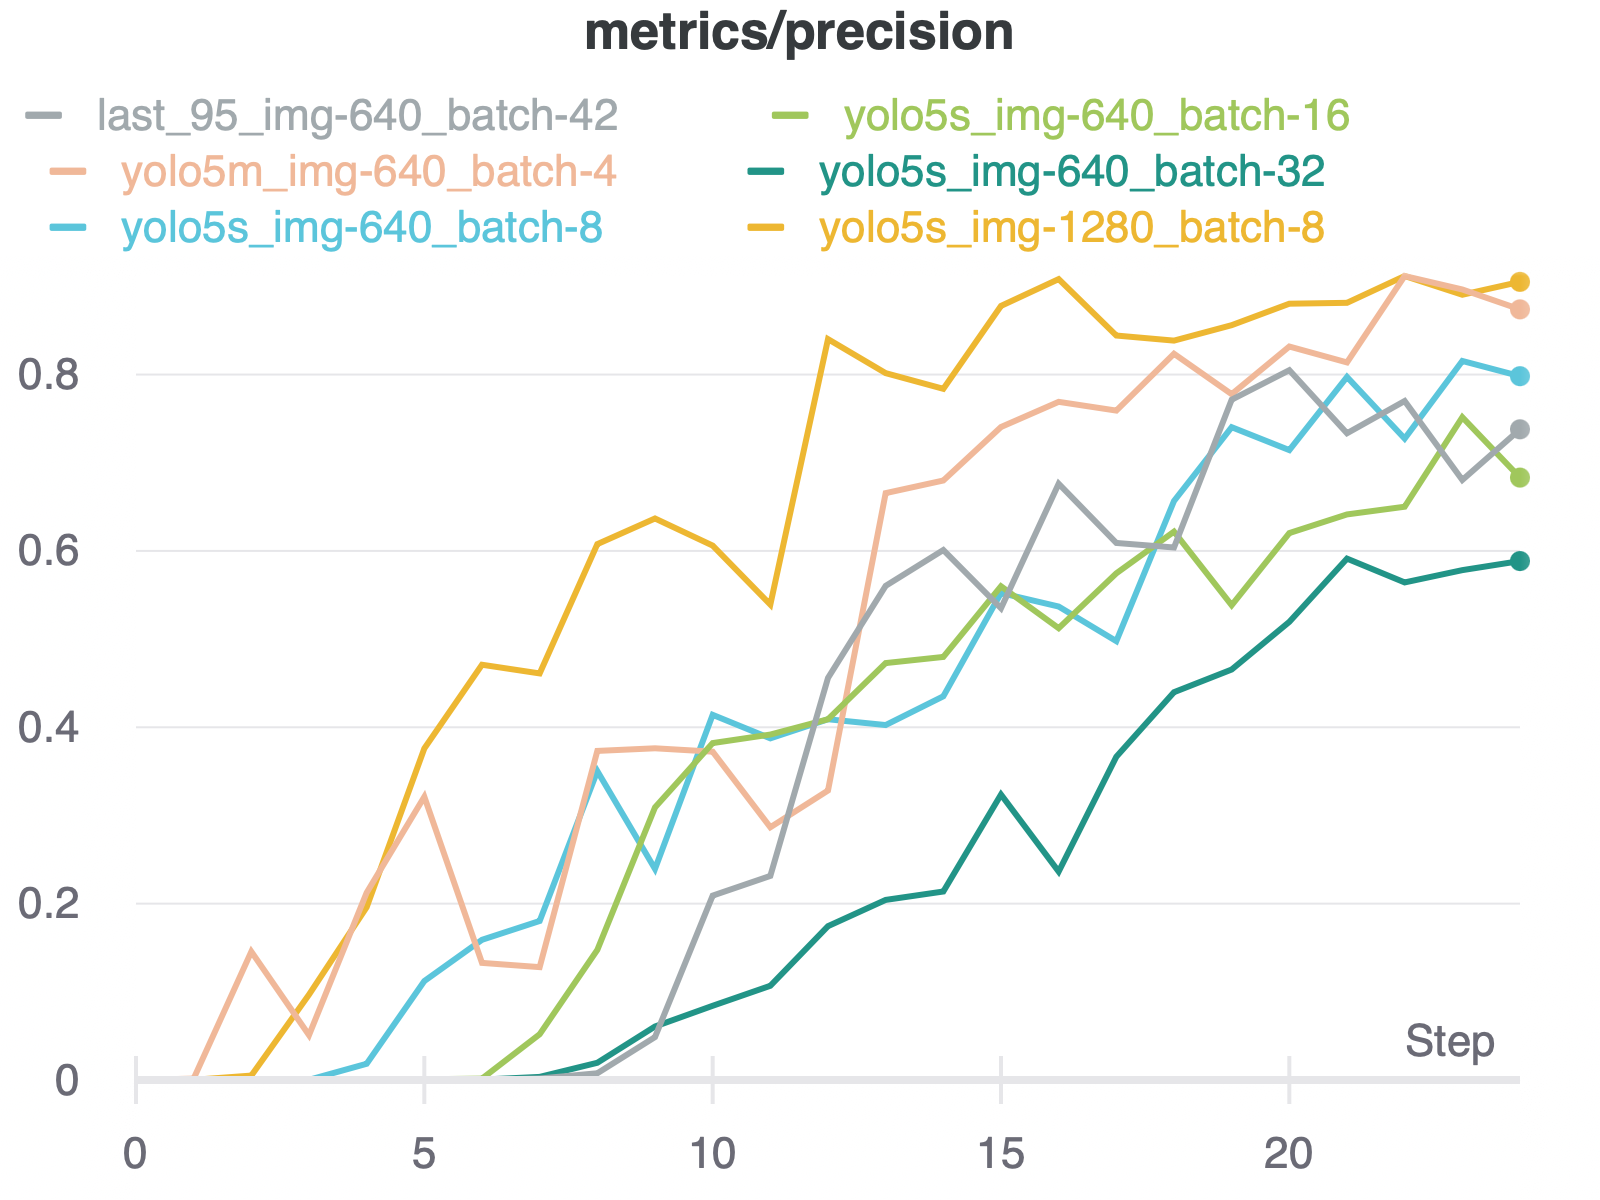
\includegraphics[height=4cm,keepaspectratio]{images/5_multimodal_fusion/exp-1_precision.png}
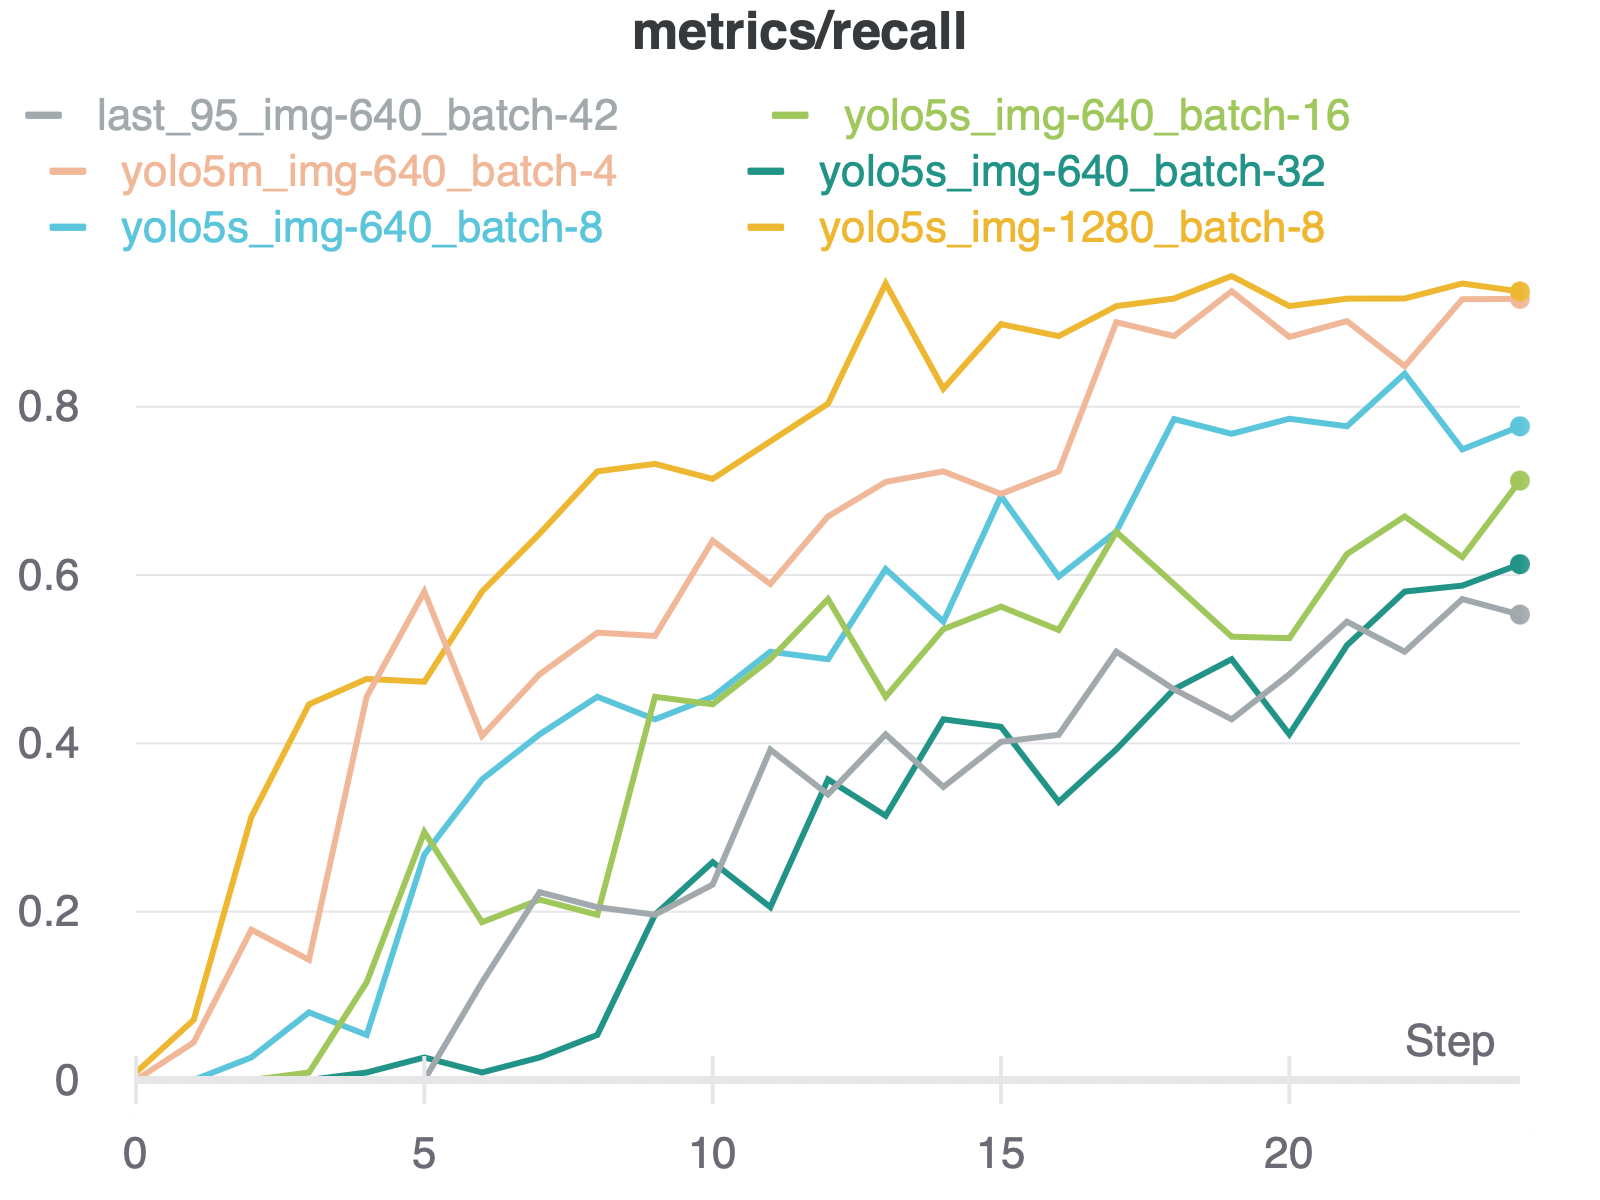
\includegraphics[height=4cm,keepaspectratio]{images/5_multimodal_fusion/exp-1_recall.png}
\end{center}
\caption{Experiment 1: performance metrics for detecting roadside location markers.}
\end{figure}


\textit{TODO: Describe the mislabelling and lower (omitted) mAP @ 0.5 scores}

\begin{figure}[h]
\begin{center}
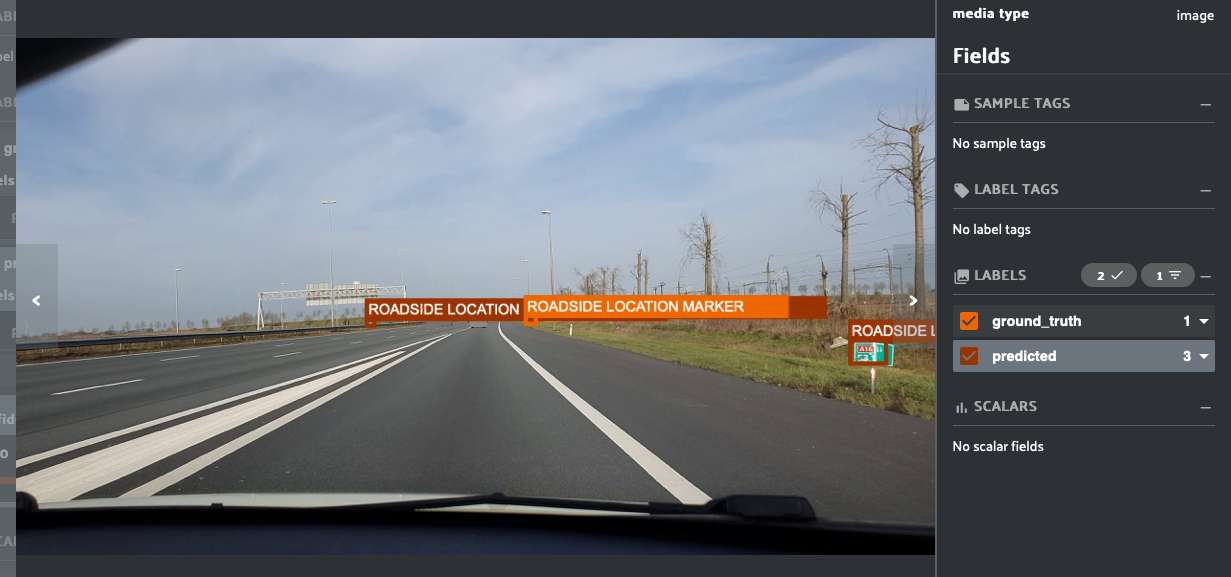
\includegraphics[width=\textwidth,keepaspectratio]{images/5_multimodal_fusion/exp-1_sample.png}
\end{center}
\caption{Example of predicted bounding boxes. Predicted boxes are in dark brown, while the ground truth labelling is in orange.}
\end{figure}

\subsubsection{Conclusion}

Detecting roadside location markers appears to be a relatively easy task for YOLO. From the results table above we see that larger models perform better. In our task this seems explainable. The roadside location marker is relatively small in the whole image. Thus, a model with larger image size works best to detect these small objects.

Although it is a simple experiment, during tests it appeared that the GPU might be a limiting factor for testing really large models. For completion, the aim was to test all possible configurations with YOLOv5s, YOLOv5m and image sizes in [640, 1280], and batch sizes in [4, 8, 16, 32]. Upon testing larger models (e.g. YOLOv5Mm with image size 1280), unfortunately the GPU experienced out of memory issues.


\subsection{ADR Cycle 2: Estimate Vehicle-to-Object Distance }

\subsection{ADR Cycle 3: Synchronize Visual and Accelerometer}

\subsection{ADR Cycle 4: Train End-to-End Multimodal DL Model}








